\chapter{Introduction}
\label{chap:introduction}
\begin{comment}
\begin{figure}[t]
    \centering
    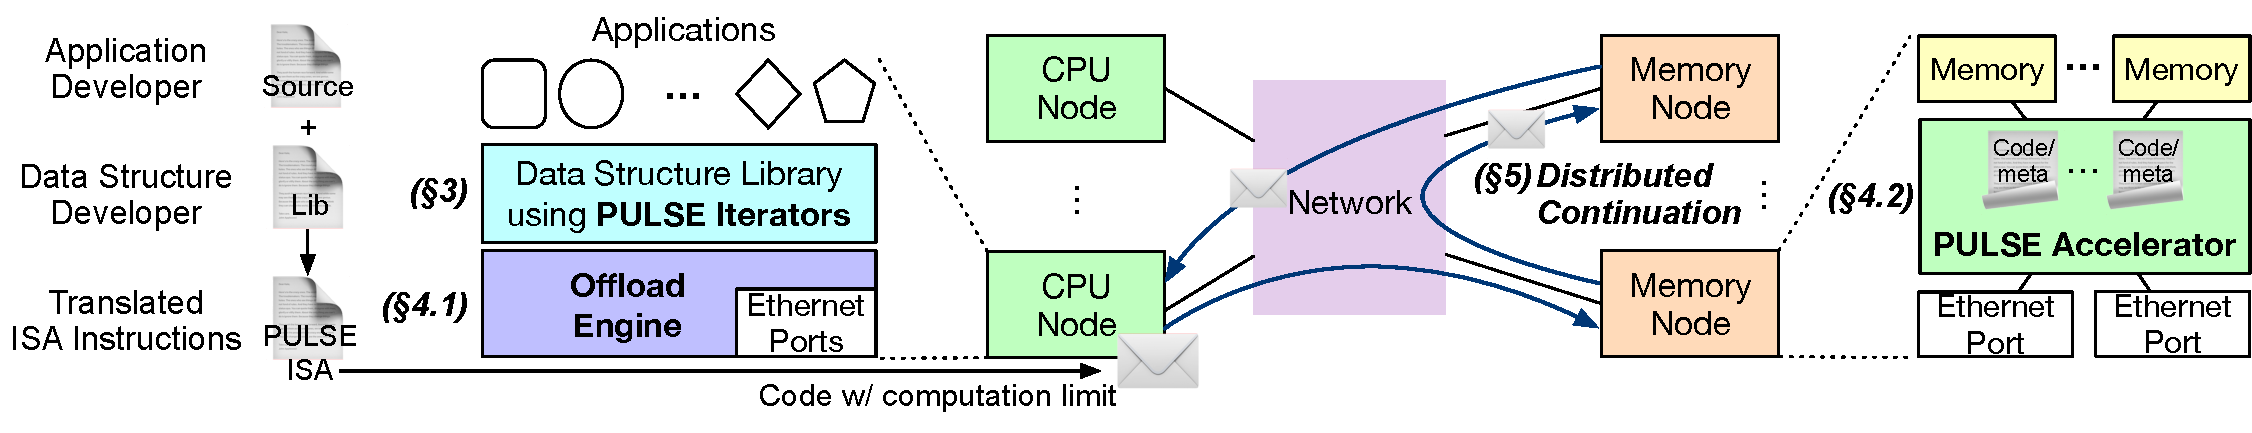
\includegraphics[width=0.8\columnwidth]{overview.pdf}
      \caption{\textbf{Cloud Stack of Disaggregated Architecture.}} \vspace{-1.0em}
      \label{fig:disagg}
\end{figure}
\end{comment}
The increasing demand for scalable and efficient data center architectures has given rise to the concept of resource disaggregation~\cite{mind, legoos}. This contemporary paradigm represents a significant departure from traditional monolithic server architectures. In conventional setups, servers typically come pre-equipped with a fixed combination of compute, memory, and storage resources. In contrast, resource-disaggregated systems physically separate these resources and distribute them across various interconnects, such as networks~\cite{disagg}, CXL~\cite{cxl}, and others. This separation fosters more flexible resource allocation and utilization.

Within the broader context of resource disaggregation in modern data center architectures, memory disaggregation~\cite{memdisagg1, memdisagg2, memdisagg3, memdisagg4, memdisagg5, memdisagg6} plays a pivotal and foundational role. Memory often serves as a bottleneck in traditional monolithic server configurations, limiting the scalability and adaptability of applications. Data centers can achieve increased efficiency, scalability, and adaptability by decoupling memory resources from compute and storage elements and presenting them as pooled, disaggregated resources. Memory-intensive workloads can access the memory they require on demand without being constrained by the limitations of individual servers. Memory disaggregation serves as the initial step toward unlocking the full potential of resource disaggregation, enabling data centers to allocate and utilize resources based on dynamic application needs efficiently. This ultimately leads to improved performance and resource utilization.

While resource disaggregation offers numerous advantages, transitioning existing applications to a disaggregated architecture is far from straightforward. Recent research efforts have explored various approaches to tackle this challenge. Some have focused on adapting applications to optimize their utilization of disaggregated memory~\cite{farm, aifm}, while others have aimed to transparently port applications and shift the responsibility of mitigating the performance penalty caused by the mismatch between disaggregated architecture and software interfaces to the service or operating system layer~\cite{mind, legoos, fastswap, infiniswap}. 

The fundamental challenge is the mismatch between the existing cloud stack for monolithic architecture and what is required for disaggregated architecture(Figure \ref{fig:disagg}). The current cloud stack and hardware stack lack awareness of the unique characteristics of disaggregated memory. There are different requirements and challenges of different layers of the stack:


\paragraphb{Application interface} In disaggregated architectures, applications face unique challenges compared to traditional monolithic systems. The primary difference is resource distribution: compute, memory, and storage are spread across multiple nodes instead of centralized in one server. This requires complex communication and data management strategies to handle increased latency and resource management needs. In contrast, monolithic architectures offer integrated resources, simplifying application interaction. Adapting to disaggregated systems involves significantly redesigning applications for effective resource utilization and management.

\paragraphb{OS support} Unlike monolithic servers where the OS manages resources within a single server, the placement and function of the OS in disaggregated architectures are still subjects of debate in both industry and academia. Options include centralizing the OS at a single point~\cite{mind} in the architecture or disaggregating its functions across different resource blades~\cite{legoos}.

\paragraphb{Performance overheads of disaggregation} Transitioning existing applications to a disaggregated architecture transparently introduces a spectrum of performance challenges. These include, but are not limited to, managing memory partitioning~\cite{jiffy} and addressing applications with irregular memory access patterns~\cite{chase}. Various other issues, such as latency sensitivity, bandwidth limitations, and the overhead of remote resource management, compound this complexity. These factors contribute to the overall performance penalty that disaggregated systems must carefully consider and mitigate.

\paragraphb{Future interconnects} Using networks as interconnects for resource disaggregation has been a subject of exploration in academia and industry. However, networks have inherent challenges, such as performance slowdowns compared to intra-server resource access and a lack of inherent coherency. Advanced hardware technologies like Compute Express Link (CXL)~\cite{cxl} offer promising enhancements with faster access times and hardware-supported cache coherence. Yet, the current state of hardware prototypes and software support for these technologies remains limited.

\section{Thesis Overview}

In this dissertation, we attempt to take a top-down approach and explore the solutions for each layer of disaggregated memory architectures. We focus on memory management challenges.

\subsection{Elastic Memory Management for Data Analytics}
\subsection{In-Network Memory Management for Disaggregated Data Centers}
\subsection{Accelerating Distributed Pointer-traversals}
\subsection{Exploring Performance and Cost Optimization with ASIC-Based CXL Memory}

\section{Outline and Previously Published Work}

This dissertation is organized as follows. Chapter~\ref{chap:service} introduces Jiffy, a distributed memory management system that decouples memory capacity and lifetime from compute in the serverless paradigm. Chapter~\ref{chap:os} describes two innovated system design: (1) MIND, a rack-scale memory disaggregation system that uses programmable switches to embed memory management logic in
the network fabric. (2) PULSE, a framework centered on enhancing in-network optimizations for
irregular memory accesses within disaggregated data centers. Chapter ~\ref{chap:hardware} presents our exploration in latest Compute Express Link(CXL) hardware. We conclude with our contributions and possible future work directions in Chapter~\ref{chap:future}.

Chapter~\ref{chap:service} revises material from ~\cite{jiffy}. Chapter~\ref{chap:os} revises material from ~\cite{mind} and ~\cite{chase}. Finally, Chapter~\ref{chap:hardware} revises material from ~\cite{cxleurosys}.
